\chapter{Registro de mudanças no processo}


\begin{table*}[!h]
\centering
\caption{Mudanças no processo de Engenharia de Requisitos}
\label{Rotulo}
  \begin{tabular}{p{0.20\linewidth}p{0.25\linewidth}p{0.25\linewidth}}
  \hline
  Data  & Processos mudados & Versão Gerada\\
  \hline

  23/05/2015 & Macroprocesso e Subprocesso Executar Iteração & 2.0\\

  04/06/2015  & Macroprocesso & 3.0 \\

  \hline
  \end{tabular}
\end{table*}

Na versão 1.0 do processo, Figuras \ref{fig:Processo1} e \ref{fig:iteracao1}, atividades de gerência de mudanças e alguns \textit{gateways} foram acrescentados, também foi retirado o subprocesso
  Executar Release. Essas mudanças foram realizadas pois não havia um fluxo definido para quando
  surgissem novos Requisitos ao longo do processo e também não havia o relacionamento de volta entre os níveis do SAFe. O subprocesso foi retirado
  pois ele foi transformado em atividades no macroprocesso que seguiam a ordem correta de execução.

Assim a mudança ocorrida possui as seguintes informações:
\begin{figure}[!htb]
\flushleft
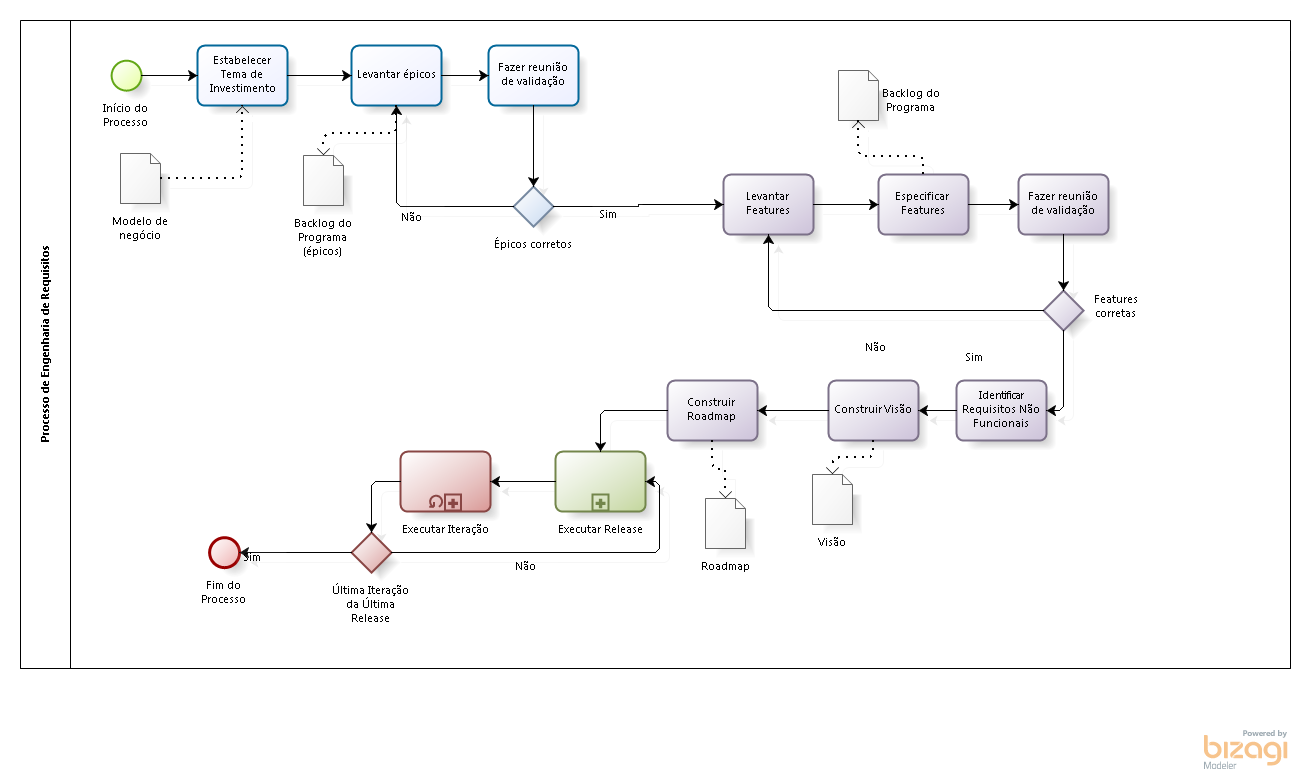
\includegraphics[scale=0.5]{figuras/processo1.png}
\caption{Processo de Engenharia de Requisitos - Versão 1.0}
\label{fig:Processo1}
\end{figure}

\begin{figure}[!htb]
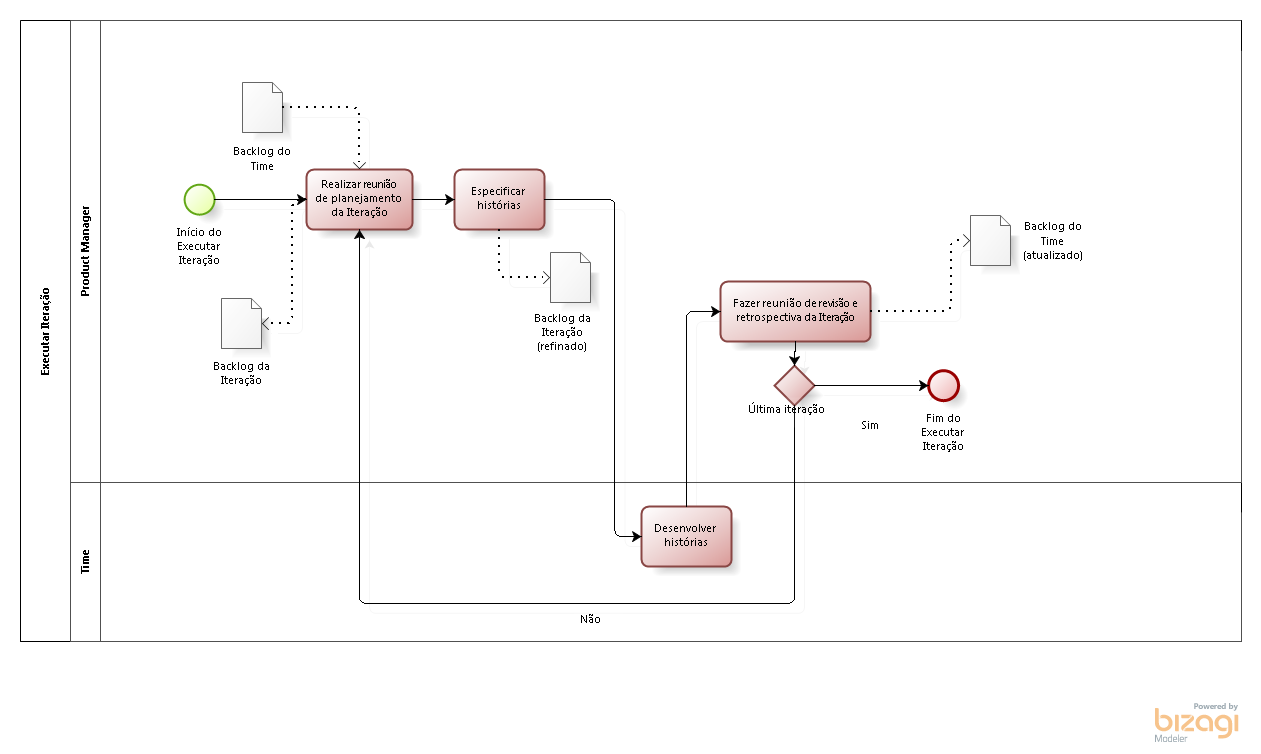
\includegraphics[scale=0.5]{figuras/iteracao1.png}
\caption{Suprocesso Executar Iteração - Versão 1.0}
\label{fig:iteracao1}
\end{figure}

Na versão 2.0 do processo, Figura \ref{fig:Processo2}, atividades de validação dos épicos e \textit{features} foram mescladas às atividades de elicitação desses requisitos.
Essa mudança foi realizada, pois foi percebida que essas atividades poderiam ser tarefas, visto que em outros momentos do processo foi estabelecido assim.\\

\begin{figure}[!htb]
\flushleft
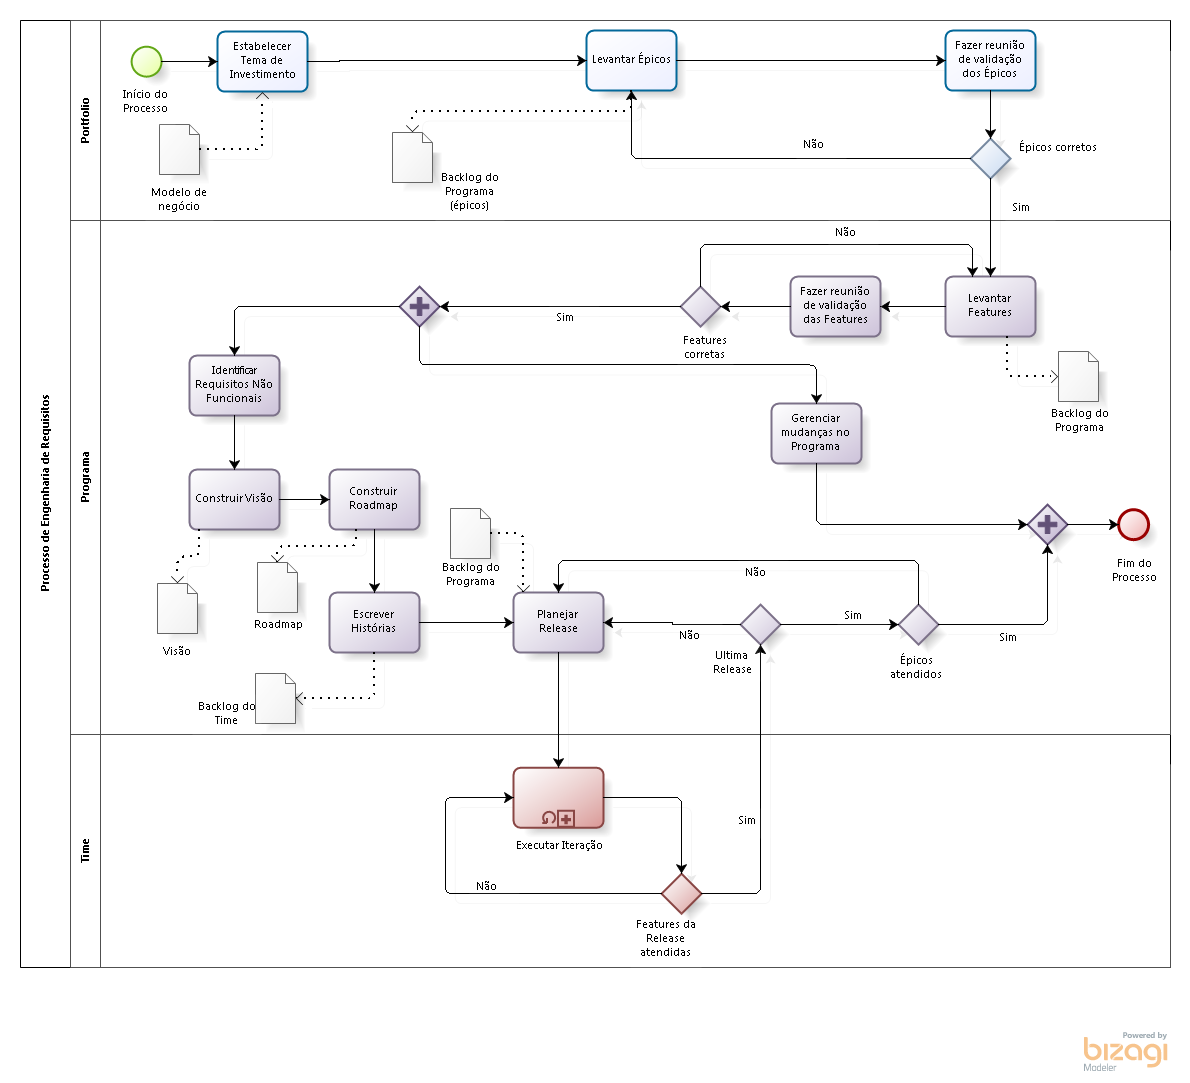
\includegraphics[scale=0.5]{figuras/processo2.png}
\caption{Processo de Engenharia de Requisitos - Versão 2.0}
\label{fig:Processo2}
\end{figure}
